\documentclass[tikz, border=5pt]{standalone}
\usetikzlibrary{perspective, arrows.meta}

\begin{document}

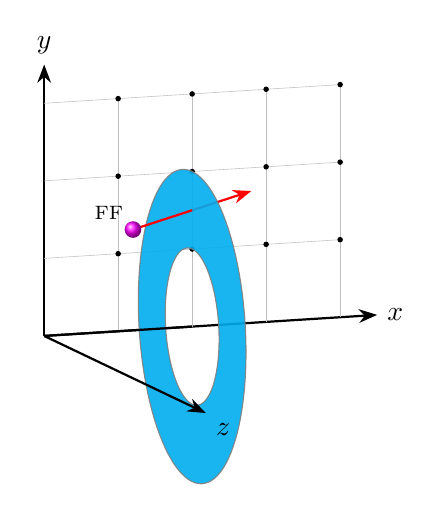
\begin{tikzpicture}[3d view={70}{10}, >=Stealth]
	% zxy (labels) is actually xyz (tikz cs)
	% \draw[->, thick] (0, 0, 0) -- (6.0, 0, 0) node[below right] {$z$};
	\draw[->, thick] (0, 0, 0) -- (0, 4.5, 0) node[right] {$x$};
	\draw[->, thick] (0, 0, 0) -- (0, 0, 3.5) node[above] {$y$};

	\foreach \y in {1,...,4}
		\foreach \z in {1,...,3} {
			\draw[gray!50, very thin]
				(0, \y, \z) -- (0, \y, \z - 1);
			\draw[gray!50, very thin]
				(0, \y, \z) -- (0, \y - 1, \z);
		}

	\foreach \y in {1,...,4}
		\foreach \z in {1,...,3} {
			\fill (0, \y, \z) circle [radius=1pt];
		}

	\draw[->, red, thick] (0, 2.0, 1.5) -- (0, 2.8, 1.7);

	\draw[color=gray, fill=cyan, opacity=0.9, even odd rule]
		plot[domain=0:360, samples=100] ({2*cos(\x)}, 2, {2*sin(\x)}) --cycle
		plot[domain=0:360, samples=100] ({1*cos(\x)}, 2, {1*sin(\x)}) --cycle;

	\draw[red, thick] (0, 1.2, 1.3) -- (0, 2.0, 1.5);
	\shade[ball color=magenta]
		(0, 1.2, 1.3) circle [radius=3pt]
		node [above left, font=\scriptsize] {FF};

	% redrawing things because of z-order
	\draw[thick] (0, 0, 0) -- (0, 2, 0);
	\draw[->, thick] (0, 0, 0) -- (6.0, 0, 0) node[below right] {$z$};

\end{tikzpicture}

\end{document}
